\aberturaModulo{MÓDULO 4}{INDICADORES AMBIENTAIS, QUALIDADE DO SOLO E DIAGNÓSTICO DE DEGRADAÇÃO}{Semanas 11 a 13 $\bullet$ Atividade de Campo no Semiárido e Base Técnica do Diagnóstico Final}{%
Este módulo marca a passagem do diagnóstico estrutural da paisagem (bacias, morfopedologia, geossistemas e fragilidade) para a \textbf{medição quantitativa, o monitoramento em campo e a avaliação operacional da degradação ambiental}. Os três capítulos articulam diretamente a viagem de campo no Semiárido Baiano e fornecem o núcleo técnico-metodológico para o Trabalho Prático Final da disciplina CHF662:
\begin{itemize}[leftmargin=1.5em, itemsep=3pt]
  \item \textbf{Capítulo 10, Indicadores Ambientais, Monitoramento e Análise de Campo no Semiárido Baiano (Semana 11):} critérios de seleção de indicadores (Fidalgo, 2003; IBGE, 2018; OECD, 2003), matrizes PER/PEIR e estudo integrado da inserção eólica e energética em Canudos e no Submédio São Francisco (Paulo Afonso, Rodelas, Sobradinho, Casa Nova, Sento Sé e Juazeiro).
  \item \textbf{Capítulo 11, Indicadores de Qualidade do Solo e Funcionalidade Edáfica (Semana 12):} atributos físicos, químicos e biológicos, Conjunto Mínimo de Dados (MDS), fator de van Bemmelen, normalização (0 a 1) e cálculo passo a passo do Índice de Qualidade do Solo (IQS).
  \item \textbf{Capítulo 12, Diagnóstico de Processos de Degradação Ambiental e Erosão Linear (Semana 13):} evolução hídrica do salpicamento (\textit{splash}) à voçoroca, \textit{piping}, Equação Universal de Perda de Solo (USLE), assoreamento de reservatórios e monitoramento em campo com pinos de erosão e perfis transversais.
  \item \textbf{Simulado e Revisão Integrada do Módulo 4:} oito questões objetivas autorais no estilo ENADE e concursos ambientais, duas questões dissertativas aplicadas, gabarito comentado, espelho de correção e quadro de autoavaliação.
\end{itemize}
}

\chapter{Indicadores Ambientais, Monitoramento e Análise de Campo no Semiárido Baiano}
\label{cap:indicadores_peir_semiarido}

\noindent\tagCampo\ \tagPratica
\vspace{4pt}

\begin{capObjetivos}
Ao concluir este capítulo, você será capaz de:
\begin{itemize}[leftmargin=1.5em, itemsep=2.5pt]
  \item Distinguir dado bruto, parâmetro, variável, indicador e índice na análise ambiental aplicada.
  \item Selecionar indicadores ambientais segundo critérios internacionais de relevância política e técnica, solidez analítica, mensurabilidade e sensibilidade (OECD, 2003; Fidalgo, 2003; IBGE, 2018).
  \item Estruturar passo a passo matrizes nos modelos Pressão--Estado--Resposta (PER) e Pressão--Estado--Impacto--Resposta (PEIR), estabelecendo nexos causais verificáveis entre vetores antrópicos e respostas de gestão.
  \item Analisar criticamente a inserção da matriz eólica na região de Canudos e no eixo energético do Submédio São Francisco (Paulo Afonso, Rodelas, Sobradinho, Casa Nova, Sento Sé e Juazeiro), relacionando viabilidade locacional, conservação da Caatinga, erosão em acessos, avifauna e usos múltiplos da água.
  \item Calcular métricas de campo e monitoramento aplicáveis a relatórios técnicos, como taxa de supressão vegetal, densidade viária de serviços, variação de vazão regularizada e estimativa corrigida de mortalidade de avifauna.
\end{itemize}
\end{capObjetivos}

\begin{capRevisao}
Para acompanhar com segurança a construção de matrizes de indicadores e o estudo de campo no Semiárido, retome os seguintes fundamentos desenvolvidos nos módulos anteriores:
\begin{itemize}[leftmargin=1.5em, itemsep=2.5pt]
  \item \textbf{Aspecto ambiental, impacto e mitigação (Capítulos 4 e 5):} aspecto é o elemento de uma atividade que interage com o meio (por exemplo, supressão vegetal para abertura de acesso); impacto é a alteração mensurável decorrente dessa interação (erosão em talude, fragmentação de habitat).
  \item \textbf{Escalas espaciais e análise integrada (Capítulo 6):} empreendimentos energéticos operam simultaneamente na escala local (base de torre e talude), na escala de microbacia (escoamento e assoreamento) e na escala regional (corredores eólicos e regularização hidrelétrica do Rio São Francisco).
  \item \textbf{Bacias hidrográficas, morfopedologia e fragilidade ambiental (Capítulos 7 a 9):} chapadas, serras residuais e pedimentos semiáridos exibem solos rasos (Neossolos Litólicos, Planossolos e Luvissolos) cuja retirada da cobertura da Caatinga eleva abruptamente a fragilidade emergente de Ross (1994).
\end{itemize}
\end{capRevisao}

\etapa{3}{Fundamentação Teórica: Indicadores Ambientais, Modelo PEIR e Campo no Semiárido}

\begin{boxSimbolo}[Vocabulário Técnico e Símbolos do Capítulo 10]
O \textbf{dado bruto} corresponde a uma observação ou contagem isolada obtida em campo, laboratório ou sensoriamento remoto, como registrar $12$ focos erosivos em uma estrada ou medir $18{,}0\text{ ha}$ de vegetação removida. Quando essa grandeza é relativizada por uma base espacial ou temporal e ligada a um objetivo de gestão, ela opera como um \textbf{indicador ambiental}, a exemplo da densidade de focos por quilômetro ($\text{focos}\cdot\text{km}^{-1}$). A agregação matemática de dois ou mais indicadores padronizados em uma métrica composta única gera um \textbf{índice ambiental}, como o Índice de Qualidade do Solo ou o Índice de Qualidade da Água. Nas equações operacionais deste capítulo, $A_{\text{sup}}$ designa a área suprimida ($\text{ha}$), $T_{\text{sup}}$ expressa a taxa percentual de supressão ($\%$), $D_v$ representa a densidade viária ($\text{km}\cdot\text{km}^{-2}$), e $M_{\text{est}}$ indica a mortalidade estimada de avifauna corrigida pela eficiência de busca ($e$) e pela persistência de carcaças ($p$).
\end{boxSimbolo}

\section{Dados, Indicadores, Índices e Pirâmide da Informação Ambiental}

No trabalho geográfico e na gestão ambiental, a abundância de dados não equivale automaticamente à qualidade do diagnóstico. Um relatório técnico repleto de tabelas desconexas pouco orienta o tomador de decisão se as variáveis não responderem a perguntas ambientais precisas. Contar $12$ focos erosivos em $2\text{ km}$ de estrada revela uma degradação muito mais severa do que contar os mesmos $12$ focos distribuídos ao longo de $40\text{ km}$. A ponte entre a medição bruta em campo e a decisão territorial é construída pelos \textbf{indicadores ambientais}.

Segundo a Organização para a Cooperação e Desenvolvimento Econômico (OECD, 2003), um indicador é um parâmetro, ou valor derivado de parâmetros, que descreve o estado de um fenômeno ou de uma área com significado que ultrapassa o valor isolado da grandeza medida. No Brasil, o IBGE (2018) e Fidalgo (2003) ressaltam que um indicador bem selecionado cumpre três funções operacionais interligadas: simplifica processos socioambientais complexos em grandezas comparáveis no espaço e no tempo, garante quantificação e rastreabilidade documental da fonte e do método de coleta, e comunica evidências objetivas para comunidades locais, conselhos de bacia e órgãos ambientais (como INEMA e IBAMA).

A informação ambiental percorre três degraus progressivos de síntese crescente, da coleta primária à tomada de decisão (Figura~\ref{fig:piramide_informacao}). Na base ficam os \textbf{dados brutos} obtidos em cadernetas de campo, estações hidrométricas ou imagens orbitais; no nível intermediário, os \textbf{indicadores} relativizam essas medições por área, tempo ou meta de referência; no topo, os \textbf{índices compostos} agregam múltiplos indicadores normalizados para apoiar decisões estratégicas, exigindo sempre o reporte dos componentes individuais para que uma média favorável em um atributo não mascare gargalos críticos em outro.

\begin{figure}[H]
  \centering
  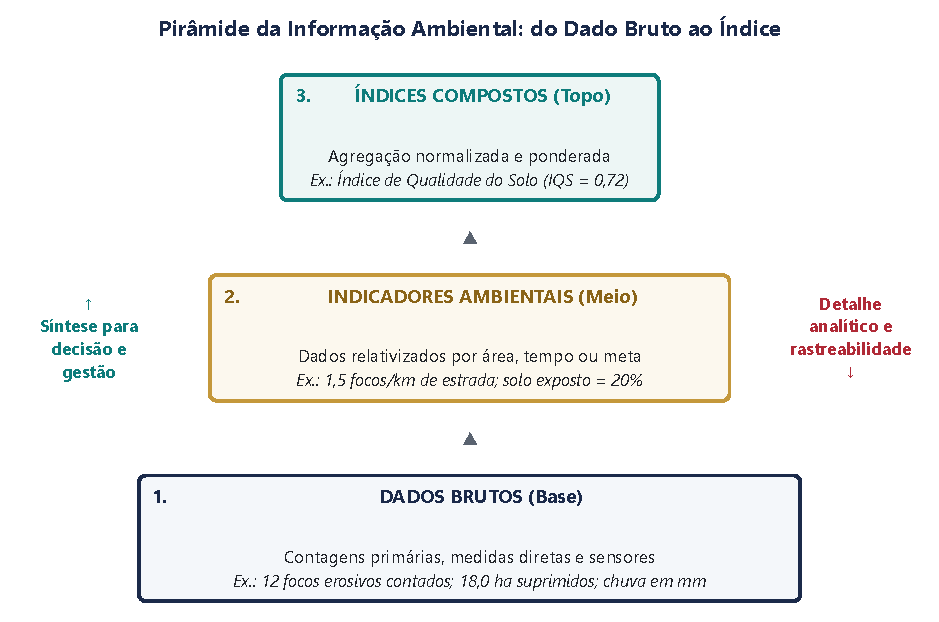
\includegraphics[width=0.90\textwidth]{figures/fig_cap10_piramide_informacao.pdf}
  \caption{Pirâmide da informação ambiental, ilustrando a passagem do dado bruto coletado em campo ao indicador relativizado e ao índice composto de decisão.}
  \label{fig:piramide_informacao}
\end{figure}

\section{Critérios de Seleção de Indicadores Ambientais}

Para evitar a escolha arbitrária de variáveis caras ou pouco informativas, OECD (2003), Fidalgo (2003) e IBGE (2018) consolidam quatro critérios de seleção que todo indicador deve atender antes de ingressar em um programa de monitoramento (Figura~\ref{fig:criterios_ocde}). A \textbf{relevância política e técnica} assegura vínculo direto com um problema concreto ou condicionante legal; a \textbf{solidez analítica} exige base científica reconhecida e protocolo repetível por técnicos independentes; a \textbf{mensurabilidade} verifica viabilidade orçamentária e regularidade temporal da série histórica; e a \textbf{sensibilidade} avalia se o indicador acusa degradação precoce e responde às intervenções corretivas em prazo útil à gestão.

\begin{figure}[H]
  \centering
  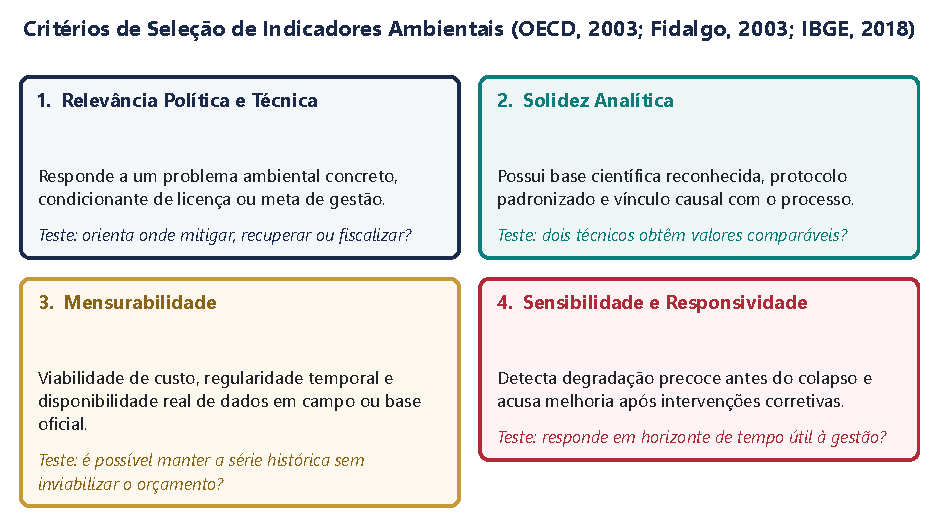
\includegraphics[width=0.92\textwidth]{figures/fig_cap10_criterios_ocde.pdf}
  \caption{Os quatro critérios de seleção de indicadores ambientais (OECD, 2003; Fidalgo, 2003; IBGE, 2018) e suas perguntas de auditoria em campo.}
  \label{fig:criterios_ocde}
\end{figure}

O Exemplo 10.1 aplica esses quatro critérios à triagem de propostas reais em um complexo eólico na Caatinga baiana.

\begin{boxExemplo}{10.1 (Básico)}{Triagem de Indicadores Ambientais segundo os Critérios da OCDE}
\passoEnunciado{Uma equipe técnica da UEFS foi convidada a propor indicadores para monitorar a conservação da Caatinga no entorno de um complexo eólico em Canudos (BA), avaliando quatro candidatos: percentual de área com solo exposto em cortes e platôs (I); percepção genérica de beleza da paisagem sem questionário padronizado (II); densidade de focos erosivos ativos por quilômetro de acesso (III); e sequenciamento genômico semanal de todos os micro-organismos do solo em 80 pontos (IV).}
\passoDados{Critérios obrigatórios de triagem (OECD, 2003; Fidalgo, 2003; IBGE, 2018): relevância política/técnica, solidez analítica, mensurabilidade e sensibilidade, avaliados como \textit{Atende (A)}, \textit{Atende parcialmente (P)} ou \textit{Não atende (N)}.}
\passoPedido{Avaliar os quatro candidatos, justificar quais devem ser selecionados e apontar o critério violado nos indicadores descartados.}
\passoMetodo{Aplicação da matriz de aderência aos quatro critérios de seleção de indicadores ambientais, verificando rigor científico, viabilidade operacional e vínculo direto com o problema de degradação.}
\passoContas{
Os \textbf{Candidatos I e III} atendem plenamente aos quatro critérios: medem proteção superficial e erosão linear com protocolo replicável em campo/imagens (A), baixo custo de repetição semestral (A) e alta sensibilidade a obras de drenagem e revegetação (A). O \textbf{Candidato II} falha em \textbf{solidez analítica (N)} e \textbf{mensurabilidade replicável (N)} por carecer de questionário estruturado e desenho amostral. O \textbf{Candidato IV} falha em \textbf{mensurabilidade operacional e financeira (N)}, com custo proibitivo e ausência de vínculo direto com a gestão de erosão.}
\passoResposta{Selecionam-se os indicadores I e III. O indicador II exige reformulação metodológica; o indicador IV é inviável para o monitoramento rotineiro proposto.}
\passoVerificacao{Os dois indicadores aprovados cobrem diretamente o estado físico da superfície e o impacto erosivo linear com orçamento realista e auditável.}
\end{boxExemplo}

\section{Modelos PER, PEIR e DPSIR: Arquitetura Causal e Construção de Matrizes}

Um conjunto de indicadores ganha força interpretativa quando organizado dentro de uma estrutura lógica que explicite causa, alteração do meio, dano e solução. O modelo \textbf{PER (Pressão--Estado--Resposta)}, formulado por Anthony Friend e David Rapport e difundido pela OCDE (OECD, 2003), parte de uma lógica de retroalimentação na qual atividades humanas exercem \textit{pressões} sobre o meio, modificam o \textit{estado} dos recursos naturais e provocam \textit{respostas} técnicas ou políticas da sociedade voltadas a conter as pressões ou recuperar o ambiente.

Posteriormente, o Programa das Nações Unidas para o Meio Ambiente (PNUMA/UNEP) refinou essa estrutura para o modelo \textbf{PEIR (Pressão--Estado--Impacto--Resposta)}, amplamente adotado pelo IBGE, MMA e órgãos estaduais brasileiros. A inclusão do compartimento \textbf{Impacto (I)} separa com nitidez a alteração biofísica do meio (\textit{Estado}) de suas consequências ecológicas, produtivas e socioambientais (\textit{Impacto}), facilitando a articulação direta com a Avaliação de Impacto Ambiental (Capítulo 5). Em estudos regionais de maior escala, o modelo \textbf{DPSIR} acrescenta ainda a categoria \textbf{Força Motriz (D)} antes da Pressão para explicitar vetores estruturais como metas nacionais de transição energética ou expansão agropecuária (Figura~\ref{fig:modelo_peir_semiarido}).

\begin{figure}[H]
  \centering
  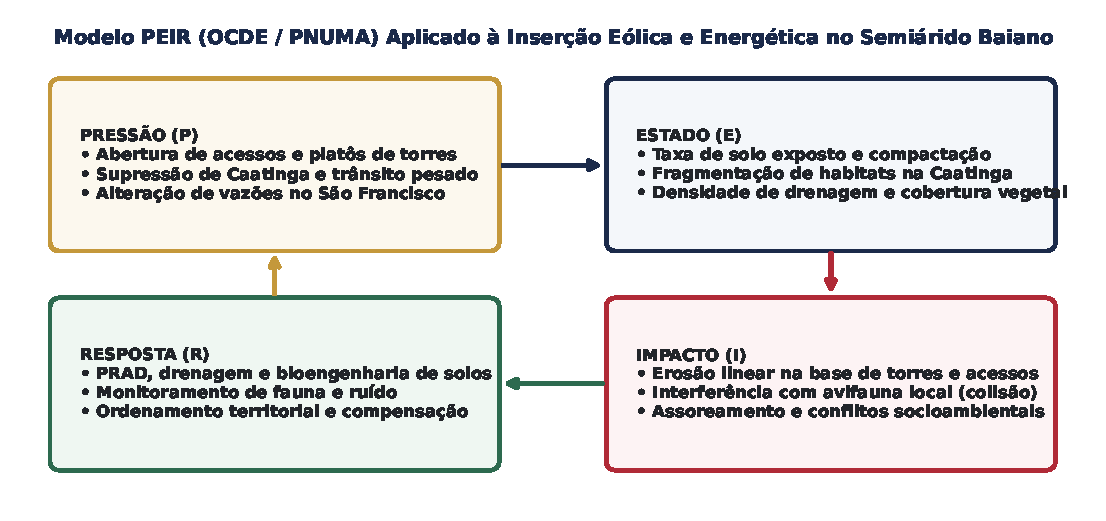
\includegraphics[width=0.94\textwidth]{figures/fig08_modelo_peir_semiarido.pdf}
  \caption{Arquitetura cíclica do modelo PEIR aplicada à inserção eólica e energética no Semiárido Baiano, integrando vetores de pressão, alterações de estado biofísico, impactos socioambientais e respostas de gestão e bioengenharia.}
  \label{fig:modelo_peir_semiarido}
\end{figure}

A leitura da Figura~\ref{fig:modelo_peir_semiarido} evidencia que o modelo PEIR opera como um \textbf{ciclo dinâmico de retroalimentação}. A \textbf{Pressão (P)} reúne ações humanas perturbadoras como a abertura de acessos e platôs ou a operação de barramentos. O \textbf{Estado (E)} retrata a condição observável dos compartimentos, como percentual de solo exposto, compactação e nível dos reservatórios. O \textbf{Impacto (I)} traduz as consequências resultantes sobre ecossistemas e comunidades, incluindo sulcos e ravinas em taludes, colisão de avifauna, assoreamento e conflitos por usos múltiplos da água. A \textbf{Resposta (R)} articula medidas corretivas e de gestão (drenagem controlada, PRAD, bioengenharia e alocação negociada em comitês de bacia), separando indicadores de execução (metros de canaleta construídos) de indicadores de resultado (redução efetiva de focos erosivos).

O Exemplo 10.3 mostra como preencher uma matriz PEIR comparando complexos eólicos e hidrelétricas ao longo do Submédio São Francisco.

\begin{boxExemplo}{10.3 (Intermediário)}{Construção de Matriz PEIR para o Eixo Energético do Submédio São Francisco}
\passoEnunciado{A partir das observações da viagem de campo entre Sobradinho, Casa Nova, Juazeiro, Rodelas e Paulo Afonso, estruture uma matriz PEIR integrando complexos eólicos em bordas de chapada e regularização hidrelétrica de vazões no Rio São Francisco.}
\passoDados{Roteiro de campo DCHF/UEFS e evidências registradas em reservatórios, calha fluvial e parques eólicos instalados sobre Caatinga hiperxerófila.}
\passoPedido{Preencher uma matriz PEIR coerente contendo Pressão, Estado, Impacto e Resposta com indicadores mensuráveis para cada vetor.}
\passoMetodo{Separação rigorosa entre atividade antrópica (P), alteração física ou biótica do compartimento (E), consequência socioambiental (I) e instrumento de gestão ou mitigação (R).}
\passoContas{
\begin{center}
\renewcommand{\arraystretch}{1.2}
\footnotesize
\begin{tabularx}{\textwidth}{@{}p{2.2cm} >{\raggedright\arraybackslash}X >{\raggedright\arraybackslash}X >{\raggedright\arraybackslash}X >{\raggedright\arraybackslash}X@{}}
  \toprule
  \rowcolor{uefsNavy}
  \textcolor{white}{\bfseries Vetor} & \textcolor{white}{\bfseries Pressão (P)} & \textcolor{white}{\bfseries Estado (E)} & \textcolor{white}{\bfseries Impacto (I)} & \textcolor{white}{\bfseries Resposta (R)} \\
  \midrule
  \textbf{Eólicas na Caatinga} & Abertura de acessos e platôs ($\text{ha}$ suprimidos; $D_v$ em $\text{km}\cdot\text{km}^{-2}$). & Solo exposto ($\%$), compactação ($D_s$) e fragmentação vegetal. & Erosão na base de torres (focos/km) e colisão de avifauna (aves/torre/ano). & Drenagem pluvial, PRAD/bioengenharia e zonas de exclusão para rotas de aves. \\
  \rowcolor{bgGray}
  \textbf{Hidrelétricas (São Francisco)} & Operação de reservatórios com redução de vazão defluente ($\text{m}^3\cdot\text{s}^{-1}$). & Alteração do pulso hidrológico, redução de lâmina d'água e bancos arenosos. & Perda de agricultura de vazante, conflitos com irrigação e degradação ripária. & Alocação negociada no CBHSF, vazão ecológica mínima e recomposição de APPs. \\
  \bottomrule
\end{tabularx}
\end{center}}
\passoResposta{A matriz PEIR articulada permite acompanhar separadamente as causas (P), as mudanças mensuráveis do meio (E), os danos ecológicos e sociais (I) e a efetividade das ações corretivas (R) nos dois eixos energéticos.}
\passoVerificacao{Cada coluna apresenta grandezas verificáveis e evita classificar uma atividade (pressão) como impacto ou um programa de monitoramento (resposta) como estado ambiental.}
\end{boxExemplo}

Ao montar uma matriz PEIR pela primeira vez, um equívoco recorrente consiste em misturar a ação humana causadora com a consequência física resultante, conforme destacado no alerta a seguir.

\begin{boxErro}[Erro 1: Confundir Dado Bruto, Pressão e Impacto na Matriz PEIR]
\textbf{Equívoco frequente:} Listar ``abertura de $18\text{ km}$ de estradas'' na coluna de Impacto (I) ou registrar ``execução de PRAD'' na coluna de Estado (E).\par
\textbf{Correção técnica:} A abertura de estradas é a ação humana geradora de perturbação, logo pertence à \textbf{Pressão (P)}. A execução do PRAD é uma intervenção corretiva da sociedade, portanto é \textbf{Resposta (R)}. O \textbf{Estado (E)} retrata a condição biofísica resultante (percentual de solo exposto), enquanto o \textbf{Impacto (I)} expressa o dano ou consequência (ravinamento em taludes, perda de biodiversidade, assoreamento).
\end{boxErro}

\section{Métricas Operacionais de Campo e Ficha do Indicador}

Para transformar observações de campo em indicadores auditáveis na matriz PEIR, empregam-se relações quantitativas com unidades explícitas acompanhadas de uma \textbf{ficha técnica padronizada}. Cada indicador deve registrar obrigatoriamente fonte dos dados, unidade de medida, período ou frequência de coleta, método de levantamento e área de referência, assegurando reprodutibilidade científica e comparação válida entre campanhas ao longo do tempo e entre setores distintos. Na ficha de cada indicador, um trecho sem vistoria constitui informação ausente, jamais valor zero, pois atribuir zero onde não houve inspeção derruba artificialmente a média calculada e mascara focos críticos de degradação.

\begin{boxFormula}[Métricas Operacionais de Campo e Monitoramento (Modelo PEIR)]
\begin{align}
  T_{\text{sup}} &= \frac{A_{\text{sup}}}{A_{\text{pol}}} \times 100\% \qquad \text{(Taxa de supressão vegetal, em \%)} \\[5pt]
  D_v &= \frac{L_{\text{acessos}}}{A_{\text{km}^2}} \qquad \text{(Densidade viária de serviço, em km}\cdot\text{km}^{-2}\text{)} \\[5pt]
  M_{\text{est}} &= \frac{N_{\text{obs}}}{e \cdot p} \qquad \text{(Mortalidade corrigida de avifauna, em aves}\cdot\text{ano}^{-1}\text{)} \\[5pt]
  \Delta_{\%} &= \frac{X_{\text{final}} - X_{\text{inicial}}}{X_{\text{inicial}}} \times 100\% \qquad \text{(Variação percentual de estado ou resposta)}
\end{align}
Nessas expressões, $A_{\text{sup}}$ é a área suprimida ($\text{ha}$) e $A_{\text{pol}}$ é a área total da poligonal ($\text{ha}$, lembrando que $1\text{ km}^2 = 100\text{ ha}$). A variável $A_{\text{km}^2}$ representa a área da poligonal em $\text{km}^2$ e $L_{\text{acessos}}$ indica a extensão total de estradas internas ($\text{km}$). Na estimativa faunística, $N_{\text{obs}}$ corresponde às carcaças encontradas em $1\text{ ano}$, $e \in (0, 1]$ expressa a eficiência do observador na busca e $p \in (0, 1]$ representa a probabilidade de a carcaça persistir no terreno sem remoção por necrófagos entre vistorias. Por fim, $\Delta_{\%}$ mede a variação relativa entre os valores inicial e final, devendo ser distinguida da variação em \textbf{pontos percentuais} (diferença direta entre taxas já expressas em porcentagem).
\end{boxFormula}

O Exemplo 10.2 demonstra o cálculo conjunto da taxa de supressão e da densidade viária em um parque eólico no Semiárido.

\begin{boxExemplo}{10.2 (Intermediário)}{Cálculo de Supressão Vegetal e Densidade Viária em Parque Eólico}
\passoEnunciado{Durante a análise do Estudo de Impacto Ambiental (EIA) de um parque eólico situado em uma chapada no eixo Canudos--Sento Sé, quantifique a taxa percentual de supressão da Caatinga e a densidade de acessos internos dentro da poligonal do empreendimento.}
\passoDados{Área total da poligonal: $A_{\text{pol}} = 1.600\text{ ha}$. Aerogeradores: $25$ torres com platô de $0{,}45\text{ ha}$ cada. Estradas internas: $L_{\text{acessos}} = 18{,}0\text{ km}$ com largura média de $10\text{ m}$. Subestação e canteiro: $2{,}75\text{ ha}$.}
\passoPedido{Calcular a área total suprimida $A_{\text{sup}}$ em hectares, a taxa percentual de supressão $T_{\text{sup}}$ e a densidade viária interna $D_v$ em $\text{km}\cdot\text{km}^{-2}$.}
\passoMetodo{Conversão homogênea de unidades métricas para hectares ($1\text{ ha} = 10.000\text{ m}^2$) e quilômetros quadrados ($1\text{ km}^2 = 100\text{ ha}$).}
\passoContas{
\textbf{Etapa 1, Área dos platôs e das estradas de acesso ($18{,}0\text{ km} = 18.000\text{ m}$):}
\[
A_{\text{platôs}} = 25 \times 0{,}45\text{ ha} = 11{,}25\text{ ha} \qquad\qquad A_{\text{acessos}} = \frac{18.000\text{ m} \times 10\text{ m}}{10.000\text{ m}^2\cdot\text{ha}^{-1}} = 18{,}00\text{ ha}
\]
\textbf{Etapa 2, Área total suprimida, taxa percentual e densidade viária ($A_{\text{km}^2} = 1.600 / 100 = 16{,}0\text{ km}^2$):}
\begin{align*}
A_{\text{sup}} &= 11{,}25 + 18{,}00 + 2{,}75 = 32{,}00\text{ ha} \\
T_{\text{sup}} &= \frac{32{,}00}{1.600} \times 100\% = 2{,}00\% \qquad D_v = \frac{18{,}0\text{ km}}{16{,}0\text{ km}^2} = 1{,}125\text{ km}\cdot\text{km}^{-2}
\end{align*}}
\passoResposta{Área total suprimida de $32{,}00\text{ ha}$, taxa de supressão de $2{,}00\%$ da poligonal e densidade viária interna de $1{,}125\text{ km}\cdot\text{km}^{-2}$.}
\passoVerificacao{Embora $2{,}00\%$ pareça um percentual reduzido em área absoluta, $56{,}25\%$ do total suprimido ($18{,}0\text{ ha}$) corresponde a corredores lineares, gerando densidade viária superior a $1\text{ km}\cdot\text{km}^{-2}$ e potencializando a fragmentação da Caatinga.}
\end{boxExemplo}

A interpretação isolada de $T_{\text{sup}}$ sem o cruzamento com $D_v$ leva frequentemente à subestimação dos impactos lineares sobre a fauna e a drenagem, conforme alertado a seguir.

\begin{boxErro}[Erro 2: Subestimar a Fragmentação ao Olhar Apenas o Percentual Total de Supressão]
\textbf{Equívoco frequente:} Concluir que uma taxa de supressão de $2\%$ em um parque eólico é ecologicamente irrelevante.\par
\textbf{Correção técnica:} Um pequeno percentual distribuído em malha viária extensa e linhas de transmissão cria centenas de metros de borda exposta, interrompe o deslocamento de fauna terrestre e concentra o escoamento superficial das chuvas torrenciais do Semiárido. Por isso, complementa-se $T_{\text{sup}}$ com métricas espaciais como a densidade viária ($D_v$).
\end{boxErro}

No monitoramento da avifauna, contar apenas carcaças visíveis subestima a mortalidade real porque parte delas passa despercebida na vegetação ($e < 1$) ou é removida por necrófagos antes da vistoria ($p < 1$). A comparação entre taxa bruta e corrigida contra o limiar de alerta, bem como a resposta quantitativa das medidas corretivas em um PRAD, pode ser visualizada diretamente na Figura~\ref{fig:mortalidade_eficacia} e detalhada no Exemplo 10.4.

\begin{figure}[H]
  \centering
  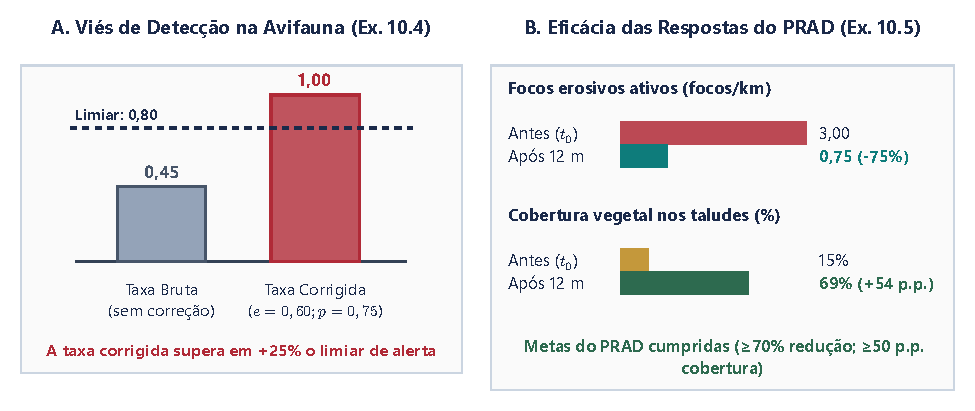
\includegraphics[width=0.92\textwidth]{figures/fig_cap10_mortalidade_eficacia.pdf}
  \caption{Comparação visual entre taxa bruta e corrigida na estimativa de mortalidade de avifauna frente ao limiar de alerta (A) e resposta quantitativa dos indicadores de recuperação após execução de PRAD (B).}
  \label{fig:mortalidade_eficacia}
\end{figure}

\begin{boxExemplo}{10.4 (Avançado)}{Indicador Corrigido de Mortalidade de Avifauna em Parque Eólico}
\passoEnunciado{O monitoramento de avifauna em um parque eólico com $40$ aerogeradores próximo a corredores ecológicos da Caatinga baiana registrou, em 12 meses de vistorias padronizadas, $18$ carcaças de aves associadas à colisão. Testes de campo indicaram eficiência de busca $e = 0{,}60$ e persistência de carcaças $p = 0{,}75$.}
\passoDados{$N_{\text{obs}} = 18$ aves/ano; $N_t = 40$ torres; $e = 0{,}60$; $p = 0{,}75$. Limiar operacional de alerta: $0{,}80\text{ ave}\cdot\text{torre}^{-1}\cdot\text{ano}^{-1}$.}
\passoPedido{Calcular a taxa bruta não corrigida por torre, a mortalidade anual estimada corrigida $M_{\text{est}}$ e a taxa corrigida por torre/ano, comparando-a ao limiar de alerta.}
\passoMetodo{Aplicação do fator de correção amostral $M_{\text{est}} = N_{\text{obs}} / (e \cdot p)$ e relativização pelo número de aerogeradores.}
\passoContas{
\begin{align*}
T_{\text{bruta}} &= \frac{18}{40} = 0{,}45\text{ ave}\cdot\text{torre}^{-1}\cdot\text{ano}^{-1} \\
e \cdot p &= 0{,}60 \times 0{,}75 = 0{,}45 \quad (\text{apenas } 45\% \text{ de detecção})
\end{align*}
\begin{align*}
M_{\text{est}} &= \frac{18}{0{,}45} = 40{,}0\text{ aves}\cdot\text{ano}^{-1} \\
T_{\text{corr}} &= \frac{40{,}0}{40} = 1{,}00\text{ ave}\cdot\text{torre}^{-1}\cdot\text{ano}^{-1}
\end{align*}
Como $1{,}00 > 0{,}80$, o limiar de alerta foi ultrapassado em $25\%$ ($\frac{1{,}00 - 0{,}80}{0{,}80}\times 100\%$).}
\passoResposta{Taxa bruta de $0{,}45\text{ ave}\cdot\text{torre}^{-1}\cdot\text{ano}^{-1}$, mas taxa corrigida de $1{,}00\text{ ave}\cdot\text{torre}^{-1}\cdot\text{ano}^{-1}$ ($M_{\text{est}} = 40$ aves/ano), superando o limiar de alerta e exigindo resposta mitigadora imediata.}
\passoVerificacao{Conforme ilustrado no Painel A da Figura~\ref{fig:mortalidade_eficacia}, a taxa bruta ocultaria a ultrapassagem do limiar caso os fatores de detecção e persistência fossem omitidos.}
\end{boxExemplo}

Sem padronização do esforço amostral e correção do viés de detecção, comparações entre campanhas perdem validade técnica.

\begin{boxErro}[Erro 3: Comparar Contagens Brutas de Fauna ou Erosão sem Padronização Amostral]
\textbf{Equívoco frequente:} Relatar apenas o número absoluto de carcaças de aves ou focos erosivos sem considerar esforço amostral, número de torres, extensão vistoriada ou eficiência de detecção.\par
\textbf{Correção técnica:} Sem relativização (por torre/ano ou por $\text{km}$ de estrada) e sem correção de viés de detecção ($e \cdot p$ no monitoramento faunístico), os números não são comparáveis entre campanhas nem entre empreendimentos, comprometendo a solidez analítica exigida pela OCDE (2003).
\end{boxErro}

\section{Estudo de Caso Integrado: Viagem de Campo no Semiárido Baiano}

A atividade de campo prevista na Semana 11 do Plano CHF662 percorre a região de \textbf{Canudos} e o eixo energético do \textbf{Submédio São Francisco}, nos municípios de \textbf{Paulo Afonso, Rodelas, Sobradinho, Casa Nova, Sento Sé e Juazeiro}, onde coexistem o bioma \textbf{Caatinga}, chapadas e serras residuais, o maior eixo hidrelétrico do Nordeste e grandes complexos eólicos e fotovoltaicos.

\subsection{Fatores Locacionais e Leitura das Infraestruturas em Campo}

A concentração de parques eólicos resulta da convergência entre o \textbf{regime de ventos alísios de sudeste e leste} (velocidades médias frequentemente entre $7{,}5$ e $9{,}5\text{ m}\cdot\text{s}^{-1}$ a $100\text{ m}$, com máxima intensidade no segundo semestre seco e complementaridade sazonal à geração hidrelétrica), o \textbf{relevo de chapadas e serras residuais} que acelera o escoamento por efeito topográfico, a \textbf{proximidade de linhas de transmissão do SIN} estruturadas a partir de Paulo Afonso e Sobradinho, e a \textbf{estrutura fundiária} com grandes imóveis e áreas de fundo de pasto.

Em campo, observa-se como os acessos e plataformas dos aerogeradores conectam a implantação elétrica à dinâmica da vertente (Figura~\ref{fig:canudos_acessos}). Superfícies expostas recebem o impacto direto das gotas de chuva, enquanto valetas e bueiros redirecionam o escoamento superficial concentrado.

\begin{figure}[H]
  \centering
  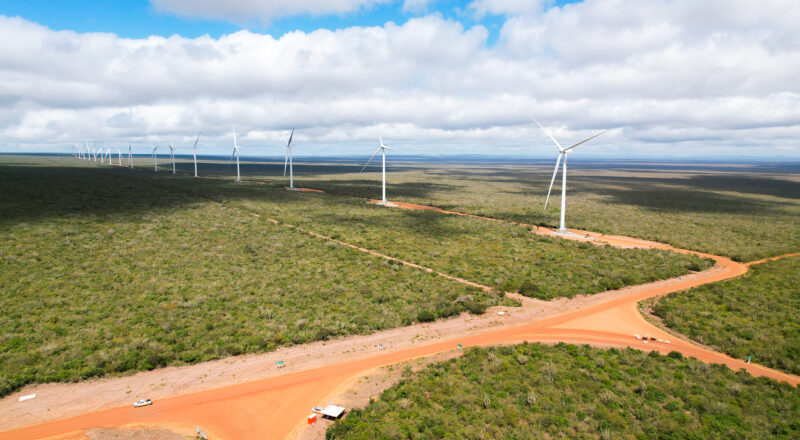
\includegraphics[width=0.78\textwidth]{figures/eolica_canudos_1.jpg}
  \caption{Aerogeradores, plataformas e acessos em área de Caatinga no eixo de Canudos. Fonte: acervo didático da disciplina.}
  \label{fig:canudos_acessos}
\end{figure}

Quando o arranjo linear das estradas de serviço atravessa divisores e unidades de drenagem, a continuidade dos corredores de solo exposto amplia a fragmentação da Caatinga e aproxima a enxurrada dos canais intermitentes (Figura~\ref{fig:canudos_linear}).

\begin{figure}[H]
  \centering
  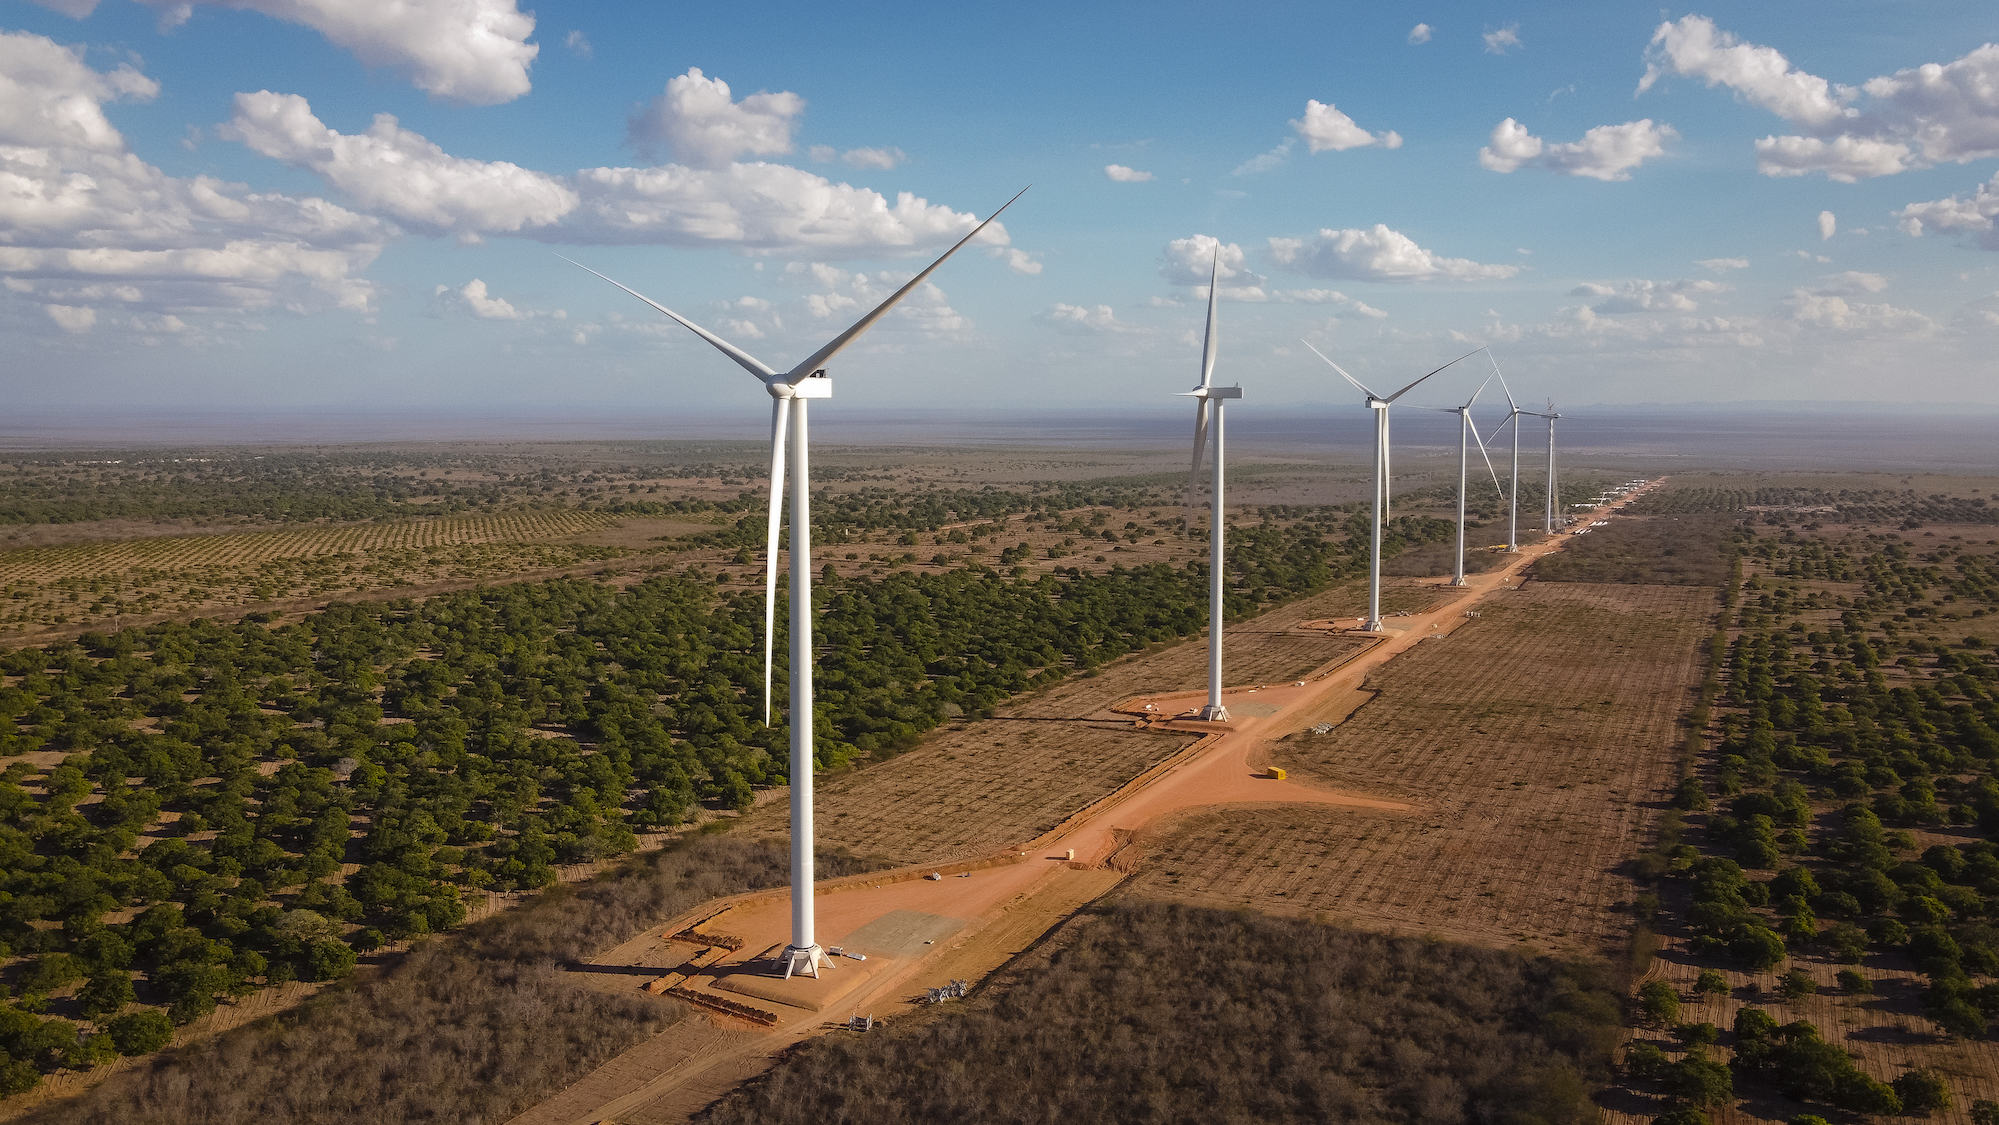
\includegraphics[width=0.78\textwidth]{figures/eolica_canudos_2.jpg}
  \caption{Arranjo linear de aerogeradores e acessos de serviço sobre superfície de solo exposto em Canudos. Fonte: acervo didático da disciplina.}
  \label{fig:canudos_linear}
\end{figure}

No eixo fluvial do Submédio São Francisco, o armazenamento hidrelétrico em Sobradinho modifica o pulso natural de cheias e vazantes, conectando geração elétrica, irrigação, abastecimento e pesca artesanal (Figura~\ref{fig:sobradinho_usina}).

\begin{figure}[H]
  \centering
  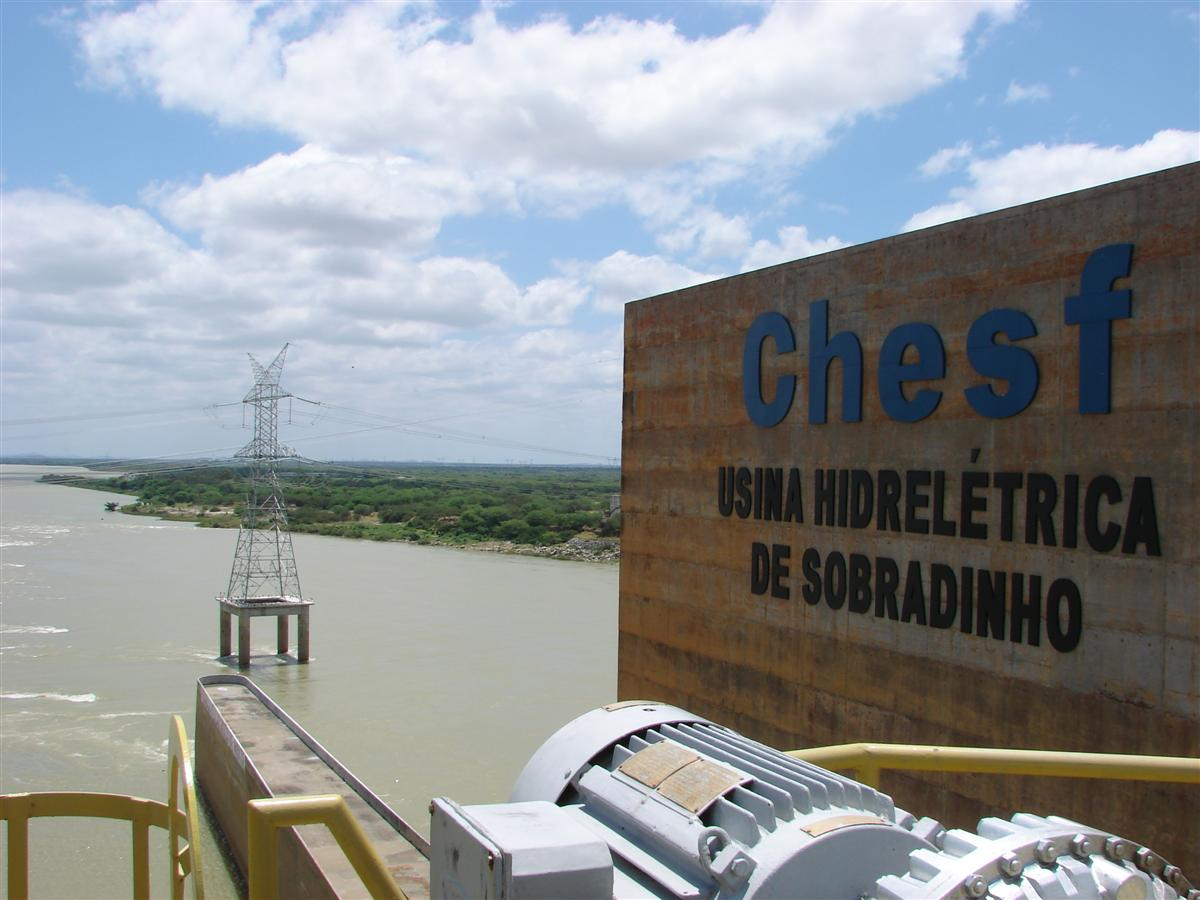
\includegraphics[width=0.78\textwidth]{figures/sobradinho_usina_glauco_umbelino.jpg}
  \caption{Usina Hidrelétrica de Sobradinho, Bahia. Fotografia de Glauco Umbelino (Wikimedia Commons, CC BY 2.0).}
  \label{fig:sobradinho_usina}
\end{figure}

Em reservatórios e chapadas semiáridas, arranjos fotovoltaicos acrescentam novas interfaces territoriais associadas à supressão vegetal em áreas planas ou à cobertura parcial do espelho d'água em sistemas flutuantes (Figura~\ref{fig:sento_se_solar}).

\begin{figure}[H]
  \centering
  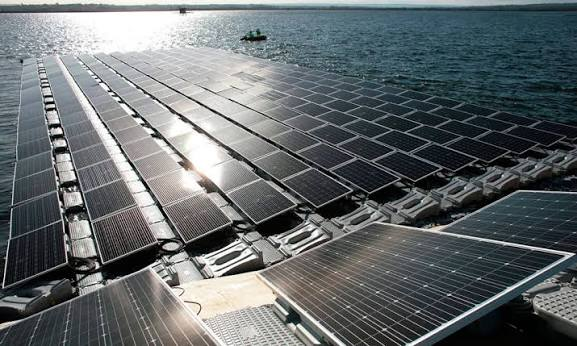
\includegraphics[width=0.78\textwidth]{figures/sento_se_solar_1.jpg}
  \caption{Módulos fotovoltaicos instalados em sistema flutuante sobre reservatório. Fonte: acervo didático da disciplina.}
  \label{fig:sento_se_solar}
\end{figure}

\subsection{Convivência com a Caatinga, Roteiro e Principais Impactos Ambientais}

A avaliação de campo no eixo Canudos--Submédio São Francisco evidencia impactos concentrados na fase de implantação e na reorganização territorial, entre os quais se destacam a supressão e a fragmentação da Caatinga por platôs e acessos para pás de $60$ a $80\text{ m}$, a erosão na base das torres e cortes de estrada em solos rasos sob chuvas convectivas concentradas, além das disputas por usos múltiplos da água diante da regularização de vazões no Rio São Francisco.

No componente faunístico, a implantação de aerogeradores e linhas de transmissão em corredores aéreos eleva o risco de colisão e cria efeito barreira para a arara-azul-de-lear (\textit{Anodorhynchus leari}), espécie endêmica e ameaçada que realiza deslocamentos diários entre os paredões areníticos usados como dormitórios e ninheiras no Raso da Catarina e as áreas de alimentação com licurizeiros (\textit{Syagrus coronata}) no entorno de Canudos (Figura~\ref{fig:arara_azul_lear}). O monitoramento contínuo das rotas de voo e o ajuste locacional de torres constituem condicionantes centrais para conciliar a geração renovável com a conservação da Caatinga.

\begin{figure}[H]
  \centering
  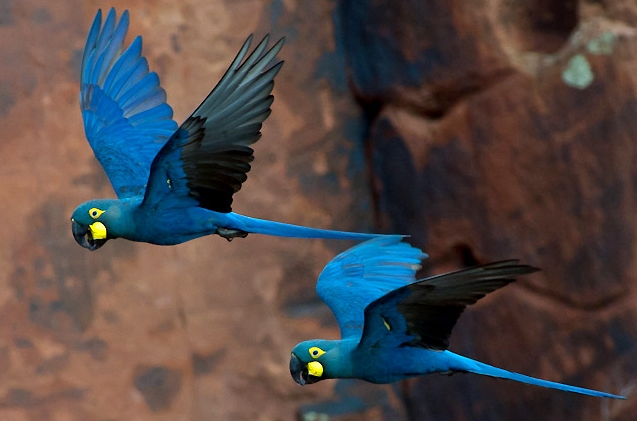
\includegraphics[width=0.76\textwidth]{figures/anodorhynchus_lear.jpg}
  \caption{Exemplares de arara-azul-de-lear (\textit{Anodorhynchus leari}) em voo junto aos paredões areníticos do Raso da Catarina, Canudos (BA), área crítica para dormitórios e corredores de forrageamento na Caatinga. Fonte: acervo didático da disciplina.}
  \label{fig:arara_azul_lear}
\end{figure}

Durante o roteiro prático, a equipe discente registra evidências georreferenciadas integrando quatro eixos: relevo e substrato (posição das torres, solos rasos e declividade), processos erosivos e drenagem (selamento, sulcos e saídas pluviais), cobertura da Caatinga e fauna (fisionomia vegetal, licurizeiros e efeito de borda) e dinâmica hídrica e socioambiental (nível dos reservatórios, irrigação e comunidades de fundo de pasto).

\etapa{4}{Avaliação de Eficácia de Respostas no Ciclo PEIR}

No fechamento do ciclo PEIR, o monitoramento pós-obra verifica quantitativamente se as ações de drenagem e revegetação cumpriram as metas estabelecidas no PRAD, como representado no Painel B da Figura~\ref{fig:mortalidade_eficacia} e calculado no Exemplo 10.5.

\begin{boxExemplo}{10.5 (Avançado)}{Avaliação Quantitativa de Eficácia de Resposta Mitigadora no Ciclo PEIR}
\passoEnunciado{Após vistoria de campo apontar erosão acelerada nos acessos de um complexo eólico no Semiárido, o empreendedor executou um programa de resposta (R) combinando canaletas revestidas, dissipadores em pedra rachão, paliçadas permeáveis e semeadura de espécies nativas da Caatinga nos taludes. Antes das obras, havia $36$ focos erosivos ativos ao longo de $12\text{ km}$ de estradas e cobertura vegetal média nos taludes de $15\%$. Doze meses após as intervenções, nova vistoria registrou $9$ focos ativos e cobertura vegetal média de $69\%$.}
\passoDados{Antes: $F_0 = 36$ focos em $12\text{ km}$; cobertura $C_0 = 15\%$. Depois (12 meses): $F_1 = 9$ focos em $12\text{ km}$; cobertura $C_1 = 69\%$. Meta contratual do PRAD: redução mínima de $70\%$ nos focos erosivos e incremento mínimo de $50$ pontos percentuais na cobertura vegetal.}
\passoPedido{Calcular a densidade inicial e final de focos erosivos, a redução percentual dos focos e o ganho absoluto (pontos percentuais) e relativo na cobertura vegetal, verificando o cumprimento das metas.}
\passoMetodo{Cálculo das razões por quilômetro de acesso e das variações absoluta e percentual entre os tempos $t_0$ e $t_1$.}
\passoContas{
\begin{align*}
D_{f,0} &= \frac{36}{12} = 3{,}00\text{ focos}\cdot\text{km}^{-1} \qquad & D_{f,1} &= \frac{9}{12} = 0{,}75\text{ foco}\cdot\text{km}^{-1} \\
\Delta F_{\%} &= \frac{9 - 36}{36} \times 100\% = -75{,}0\% & \Delta C_{\text{pp}} &= 69\% - 15\% = +54\text{ p.p.} \\
\Delta C_{\text{rel}} &= \frac{69 - 15}{15} \times 100\% = +360{,}0\% & &
\end{align*}
Conferência frente às metas: $75{,}0\% \ge 70\%$ (cumprida) e $54\text{ p.p.} \ge 50\text{ p.p.}$ (cumprida).}
\passoResposta{A densidade de focos caiu de $3{,}00$ para $0{,}75\text{ foco}\cdot\text{km}^{-1}$ (redução de $75{,}0\%$) e a cobertura vegetal avançou $+54$ pontos percentuais ($+360{,}0\%$ relativos), cumprindo ambas as metas do PRAD.}
\passoVerificacao{Distinguir \textit{pontos percentuais} ($69\% - 15\% = 54\text{ p.p.}$) de \textit{variação relativa} ($+360\%$) evita ambiguidades em auditorias ambientais, e os $9$ focos remanescentes indicam necessidade de manutenção pontual.}
\end{boxExemplo}

\etapa{5}{Armadilha Conceitual e Materiais Audiovisuais de Apoio}

Mesmo quando um empreendimento contribui para a descarbonização da matriz elétrica, o diagnóstico territorial continua indispensável para prevenir impactos locais sobre solo, água e fauna.

\begin{boxErro}[Erro 4: Assumir que Energia Eólica Equivale a Impacto Ambiental Nulo]
\textbf{Equívoco frequente:} Afirmar em diagnósticos que parques eólicos na Caatinga não causam degradação por serem fontes renováveis de baixa emissão de carbono.\par
\textbf{Correção técnica:} Toda fonte energética possui pegada territorial. No Semiárido Baiano, a implantação eólica envolve terraplenagem pesada, supressão linear da Caatinga, erosão em solos rasos de chapadas, riscos à avifauna (como a arara-azul-de-lear em Canudos) e conflitos fundiários e sonoros que exigem licenciamento rigoroso e monitoramento contínuo.
\end{boxErro}

Para aprofundar o entendimento sobre indicadores simples, índices compostos e comunicação em relatórios ambientais, assista aos vídeos selecionados na página da disciplina: \textit{Indicadores e relatórios de sustentabilidade} (\url{https://www.youtube.com/watch?v=xk-Y_YivFpU}) e \textit{Você sabe o que é o Índice de Qualidade da Água (IQA)?} (\url{https://www.youtube.com/watch?v=J2HRZjnC03w}), que exemplificam a agregação e interpretação de índices ambientais.

\etapa{6}{Exercícios de Fixação}

\subsection*{Nível Básico (Conceitos, Critérios e Modelo PEIR)}

\begin{enumerate}[leftmargin=1.8em, itemsep=6pt]
  \item Explique, com um exemplo concreto ligado ao Semiárido Baiano, a diferença entre \textbf{dado bruto}, \textbf{indicador ambiental} e \textbf{índice ambiental}.
  \espacoResolucao[1.8cm]

  \item Cite os quatro critérios principais de seleção de indicadores ambientais propostos por OECD (2003), Fidalgo (2003) e IBGE (2018), explicando o risco técnico de ignorar o critério da \textit{mensurabilidade}.
  \espacoResolucao[1.8cm]

  \item Qual é a principal diferença conceitual entre o modelo \textbf{PER} (OCDE) e o modelo \textbf{PEIR} (PNUMA/GEO)? Por que essa distinção favorece a articulação com a Avaliação de Impacto Ambiental?
  \espacoResolucao[1.8cm]

  \item Classifique cada item abaixo como \textbf{Pressão (P)}, \textbf{Estado (E)}, \textbf{Impacto (I)} ou \textbf{Resposta (R)} em um parque eólico na Caatinga: (a) abertura de $14\text{ km}$ de estradas de acesso; (b) ravina ativa de $1{,}8\text{ m}$ de profundidade na saída de bueiro; (c) percentual de solo exposto de $42\%$ no talude; (d) instalação de dissipadores de energia e revegetação com espécies nativas.
  \espacoResolucao[1.8cm]

  \item Liste três fatores locacionais geográficos que explicam a intensa concentração de parques eólicos na região de Canudos e no eixo do Submédio São Francisco (Casa Nova, Sento Sé e entorno de Sobradinho).
  \espacoResolucao[1.8cm]
\end{enumerate}

\subsection*{Nível Intermediário (Cálculos de Monitoramento e Interpretação Regional)}

\begin{enumerate}[leftmargin=1.8em, itemsep=6pt, resume]
  \item Um projeto eólico em uma poligonal de $1.200\text{ ha}$ na Bahia prevê $30$ aerogeradores com platôs de $0{,}40\text{ ha}$ cada, $12\text{ km}$ de acessos internos com $8\text{ m}$ de largura média e $2{,}4\text{ ha}$ destinados à subestação. Calcule a área total suprimida ($A_{\text{sup}}$) e a taxa percentual de supressão ($T_{\text{sup}}$).
  \espacoResolucao[2.2cm]

  \item Em um período de estiagem prolongada no Submédio São Francisco, a vazão defluente média da Usina Hidrelétrica de Sobradinho foi reduzida de $1.300\text{ m}^3\cdot\text{s}^{-1}$ para $800\text{ m}^3\cdot\text{s}^{-1}$. Calcule a variação percentual dessa vazão e cite dois impactos socioambientais diretos dessa redução ao longo do eixo Juazeiro--Rodelas--Paulo Afonso.
  \espacoResolucao[2.2cm]

  \item No monitoramento anual de avifauna de um complexo eólico com $50$ torres, registraram-se $24$ carcaças de aves. Ensaios de campo indicaram eficiência de busca $e = 0{,}80$ e persistência de carcaças $p = 0{,}60$. Calcule a mortalidade total estimada ($M_{\text{est}}$) e a taxa corrigida de mortalidade em aves por torre por ano.
  \espacoResolucao[2.2cm]

  \item Uma poligonal de empreendimento energético abrange $1.500\text{ ha}$ e contém $27\text{ km}$ de estradas internas não pavimentadas. Determine a densidade viária interna ($D_v$) em $\text{km}\cdot\text{km}^{-2}$ e discuta como esse indicador se relaciona com a erosão linear na Caatinga.
  \espacoResolucao[2.0cm]

  \item Após obras de drenagem superficial e bioengenharia nos taludes de um parque eólico, o número de focos erosivos ativos reduziu-se de $28$ para $7$ em um ano. Calcule a redução percentual obtida e classifique esse indicador dentro do modelo PEIR.
  \espacoResolucao[2.0cm]
\end{enumerate}

\subsection*{Nível Aplicado (Questões Objetivas A--E)}

\begin{enumerate}[leftmargin=1.8em, itemsep=6pt, resume]
  \item Sobre os critérios de seleção de indicadores ambientais (OECD, 2003; IBGE, 2018), assinale a alternativa correta:
  \begin{alternativas}
    \item Um indicador de alta qualidade deve dispensar qualquer protocolo padronizado, permitindo interpretações subjetivas de cada analista.
    \item A sensibilidade indica a capacidade do indicador de detectar mudanças ambientais precoces e responder às medidas de manejo em prazo útil.
    \item Indicadores compostos (índices) sempre substituem integralmente os indicadores individuais, tornando desnecessário reportar as variáveis de origem.
    \item A relevância técnica exige que o indicador utilize equipamentos laboratoriais de alto custo, independentemente da viabilidade de monitoramento contínuo.
    \item A mensurabilidade refere-se exclusivamente à possibilidade de converter variáveis qualitativas em médias aritméticas sem base amostral.
  \end{alternativas}

  \item Na matriz PEIR aplicada ao eixo energético do Submédio São Francisco, a ``implantação de um programa de monitoramento telemétrico da arara-azul-de-lear e readequação do traçado de linhas de transmissão'' corresponde ao componente:
  \begin{alternativas}
    \item Pressão (P), pois altera o cronograma financeiro do empreendimento.
    \item Estado (E), pois descreve a abundância natural da espécie na Caatinga.
    \item Impacto (I), pois representa o dano causado pelas torres ao habitat.
    \item Resposta (R), pois consiste em ação técnica e de gestão destinada a prevenir ou mitigar impactos sobre a fauna.
    \item Fator abiótico de base, externo ao ciclo PEIR.
  \end{alternativas}

  \item Um parque eólico localizado em área de $2.000\text{ ha}$ suprimiu $0{,}50\text{ ha}$ por platô em $20$ torres e abriu $15\text{ km}$ de acessos com $10\text{ m}$ de largura. Sem outras áreas suprimidas, a taxa percentual de supressão ($T_{\text{sup}}$) da poligonal é igual a:
  \begin{alternativas}
    \item $0{,}50\%$.
    \item $0{,}75\%$.
    \item $1{,}25\%$.
    \item $2{,}50\%$.
    \item $5{,}00\%$.
  \end{alternativas}

  \item Em relação aos processos físicos observados em parques eólicos implantados em chapadas e serras residuais do Semiárido Baiano, é correto afirmar que:
  \begin{alternativas}
    \item A baixa pluviosidade anual do Semiárido impede completamente a ocorrência de erosão hídrica linear na base das torres.
    \item O terraplenamento de platôs e o escoamento concentrado em estradas compactadas sobre solos rasos potencializam sulcos, ravinas e assoreamento de drenagens intermitentes.
    \item A substituição da Caatinga por solo exposto em taludes de corte reduz a energia cinética do escoamento superficial.
    \item A instalação de aerogeradores elimina a necessidade de medidas de drenagem pluvial e PRAD por se tratar de energia renovável.
    \item Os ventos alísios de sudeste são os únicos responsáveis pelo transporte de sedimentos grosseiros nos bueiros das estradas de acesso.
  \end{alternativas}

  \item Em um programa de monitoramento de colisão de avifauna com $25$ torres eólicas durante um ano, foram encontradas $15$ carcaças. Sabendo que a eficiência de busca foi $e = 0{,}50$ e a persistência de carcaças foi $p = 0{,}60$, a taxa anual corrigida de mortalidade por torre é:
  \begin{alternativas}
    \item $0{,}60\text{ ave}\cdot\text{torre}^{-1}\cdot\text{ano}^{-1}$.
    \item $1{,}20\text{ aves}\cdot\text{torre}^{-1}\cdot\text{ano}^{-1}$.
    \item $1{,}50\text{ aves}\cdot\text{torre}^{-1}\cdot\text{ano}^{-1}$.
    \item $2{,}00\text{ aves}\cdot\text{torre}^{-1}\cdot\text{ano}^{-1}$.
    \item $2{,}50\text{ aves}\cdot\text{torre}^{-1}\cdot\text{ano}^{-1}$.
  \end{alternativas}
\end{enumerate}

\etapa{7}{Questões no Estilo ENADE e Concursos Ambientais}

\begin{boxDica}[Foco de Provas, ENADE e Concursos (IBAMA / INEMA)]
Exames de Geografia e concursos para Analista Ambiental frequentemente combinam leitura crítica de matrizes PEIR com dilemas concretos da transição energética no Nordeste brasileiro. Evite respostas binárias (``energia limpa = sem impacto'' ou ``toda obra é inviável'') e demonstre domínio da diferenciação entre Pressão, Estado, Impacto e Resposta com métricas verificáveis.
\end{boxDica}

\begin{enumerate}[leftmargin=1.8em, itemsep=7pt]
  \item \textbf{[Questão Autoral, Estilo ENADE / Geografia]} A expansão da energia eólica no Semiárido Baiano, especialmente em municípios como Canudos, Sento Sé e Casa Nova, tem ampliado a participação de fontes renováveis na matriz elétrica nacional. Contudo, levantamentos de campo apontam conflitos socioambientais envolvendo fragmentação da Caatinga, erosão em estradas de acesso, ruído próximo a comunidades rurais e risco de colisão para espécies ameaçadas como a arara-azul-de-lear (\textit{Anodorhynchus leari}). À luz da Análise Ambiental integrada, avalie as afirmações a seguir:
  \begin{itemize}[leftmargin=1.4em, itemsep=2pt]
    \item[I.] A viabilidade climática da energia eólica não dispensa o planejamento locacional em escala regional para evitar corredores ecológicos críticos e áreas de uso comunal.
    \item[II.] O modelo PEIR permite distinguir claramente a abertura de acessos (Pressão), a exposição do solo (Estado), o ravinamento em taludes (Impacto) e as obras de drenagem e PRAD (Resposta).
    \item[III.] Como a área diretamente ocupada pelas fundações das torres representa pequena fração do terreno, a fragmentação gerada pela malha viária não altera a conectividade da Caatinga.
  \end{itemize}
  É correto o que se afirma em:
  \begin{alternativas}
    \item I, apenas.
    \item III, apenas.
    \item I e II, apenas.
    \item II e III, apenas.
    \item I, II e III.
  \end{alternativas}

  \item \textbf{[Questão Autoral, Estilo Concurso Analista Ambiental / INEMA-BA]} No Submédio São Francisco (trecho Sobradinho--Juazeiro--Rodelas--Paulo Afonso), a gestão ambiental enfrenta pressões simultâneas decorrentes da regularização de vazões hidrelétricas, da captação para perímetros irrigados e da expansão de infraestrutura energética. Para compor um painel estadual de monitoramento baseado no modelo PEIR, um técnico deve escolher o conjunto mais coerente de indicadores. Assinale a alternativa em que os quatro elementos correspondem, respectivamente, a \textbf{Pressão, Estado, Impacto e Resposta}:
  \begin{alternativas}
    \item Assoreamento de bancos de areia; vazão defluente reduzida; plano de bacia; perda de área de vazante.
    \item Volume captado para irrigação e operação de barramentos; nível fluviométrico e percentual de vegetação ripária; conflito por usos múltiplos da água e redução da pesca artesanal; alocação negociada de água no comitê de bacia e recomposição de APPs.
    \item Recomposição de APPs; conflito por uso da água; operação de barramentos; nível fluviométrico.
    \item Nível fluviométrico; volume captado para irrigação; recomposição de APPs; redução da pesca artesanal.
    \item Conflito por uso da água; plano de bacia; volume captado; percentual de vegetação ripária.
  \end{alternativas}

  \item \textbf{[Questão Autoral, Estilo Concurso Analista Ambiental / IBAMA]} Um órgão licenciador exigiu que um empreendimento eólico substituísse indicadores genéricos de seu Programa de Monitoramento por variáveis aderentes aos critérios da OCDE (2003). Qual proposta abaixo atende simultaneamente aos critérios de \textbf{relevância técnica, solidez analítica, mensurabilidade e sensibilidade} para monitorar processos erosivos em estradas de acesso?
  \begin{alternativas}
    \item Registro fotográfico esporádico sem coordenadas geográficas e sem escala métrica, realizado apenas quando houver reclamação de moradores.
    \item Quantificação semestral da densidade de sulcos e ravinas ativos por quilômetro de acesso ($\text{focos}\cdot\text{km}^{-1}$) e da profundidade média das incisões em seções fixas georreferenciadas, acompanhada do percentual de cobertura vegetal nos taludes.
    \item Entrevista informal anual com motoristas do parque sobre se a estrada ``parece boa ou ruim'' após as chuvas.
    \item Análise mineralógica por difração de raios X realizada semanalmente em todos os bueiros do empreendimento.
    \item Contabilização apenas da geração elétrica anual em megawatts-hora (MWh), por ser o dado de maior precisão disponível na subestação.
  \end{alternativas}
\end{enumerate}

\clearpage
\etapa{8}{Gabarito Comentado do Capítulo 10}

\begin{boxGabarito}[Resoluções Completas: Exercícios de Fixação (1 a 15)]
\begin{enumerate}[leftmargin=1.6em, itemsep=4pt]
  \item \textbf{Dado bruto} é a medição isolada sem tratamento interpretativo (ex.: $12\text{ focos}$ erosivos contados em uma estrada). \textbf{Indicador} é a variável relativizada e ligada a um objetivo de gestão (ex.: $1{,}5\text{ focos erosivos}\cdot\text{km}^{-1}$ de acesso, comparado a uma meta de controle). \textbf{Índice} é a agregação matemática de múltiplos indicadores normalizados em um número sintético único (ex.: Índice de Qualidade do Solo combinando matéria orgânica, porosidade, infiltração e densidade).
  \item Os quatro critérios são: \textbf{relevância política/técnica}, \textbf{solidez analítica}, \textbf{mensurabilidade} e \textbf{sensibilidade}. Ignorar a mensurabilidade resulta em planos de monitoramento inexequíveis na prática (custos proibitivos, ausência de dados históricos ou incapacidade de repetição temporal), gerando relatórios incompletos ou descontinuados.
  \item O modelo \textbf{PER} reúne alterações físicas do meio e suas consequências sob o guarda-chuva amplo de \textit{Estado}, ao passo que o \textbf{PEIR} desdobra o compartimento \textbf{Impacto (I)} de modo explícito. Essa separação facilita a AIA porque conecta diretamente a alteração biofísica mensurada (Estado) ao dano ecológico ou socioeconômico que exige mitigação ou compensação (Impacto).
  \item (a) \textbf{Pressão (P)}, ação antrópica geradora de perturbação; (b) \textbf{Impacto (I)}, dano erosivo linear resultante; (c) \textbf{Estado (E)}, condição atual da superfície do talude; (d) \textbf{Resposta (R)}, intervenção técnica corretiva.
  \item Três fatores principais: regime de ventos alísios de sudeste/leste constantes e intensos, complementares à sazonalidade hídrica; relevo de chapadas, patamares elevados e serras residuais que amplificam a velocidade do vento acima da rugosidade da Depressão Sertaneja; e proximidade da infraestrutura de transmissão de alta tensão do Sistema Interligado Nacional estruturada historicamente a partir das hidrelétricas de Paulo Afonso e Sobradinho.
  \item \textbf{Passo a passo:}
  Platôs: $30 \times 0{,}40\text{ ha} = 12{,}00\text{ ha}$. Acessos: $12.000\text{ m} \times 8\text{ m} = 96.000\text{ m}^2 = 9{,}60\text{ ha}$. Subestação: $2{,}40\text{ ha}$.
  Área total suprimida: $A_{\text{sup}} = 12{,}00 + 9{,}60 + 2{,}40 = \mathbf{24{,}00\text{ ha}}$.
  Taxa de supressão: $T_{\text{sup}} = (24{,}00 / 1.200) \times 100\% = \mathbf{2{,}00\%}$.
  \item \textbf{Passo a passo:}
  $\Delta_{\%} = \frac{800 - 1.300}{1.300} \times 100\% = \frac{-500}{1.300} \times 100\% \approx \mathbf{-38{,}46\%}$ (redução de $38{,}46\%$).
  Impactos diretos: restrição à agricultura de vazante e pesca artesanal, exposição de bancos arenosos com maior dificuldade de captação ribeirinha e acirramento de conflitos entre geração elétrica, perímetros irrigados e abastecimento humano.
  \item \textbf{Passo a passo:}
  Fator de detecção combinado: $e \cdot p = 0{,}80 \times 0{,}60 = 0{,}48$.
  Mortalidade total estimada: $M_{\text{est}} = 24 / 0{,}48 = \mathbf{50{,}0\text{ aves}\cdot\text{ano}^{-1}}$.
  Taxa corrigida por torre: $50{,}0 / 50 = \mathbf{1{,}00\text{ ave}\cdot\text{torre}^{-1}\cdot\text{ano}^{-1}}$.
  \item \textbf{Passo a passo:}
  Convertemos $1.500\text{ ha}$ para quilômetros quadrados: $A_{\text{km}^2} = 1.500 / 100 = 15{,}0\text{ km}^2$.
  Densidade viária: $D_v = 27 / 15{,}0 = \mathbf{1{,}80\text{ km}\cdot\text{km}^{-2}}$.
  Uma malha densa de estradas compactadas intercepta o escoamento superficial natural, reduz a infiltração e concentra enxurradas nas saídas de drenagem, desencadeando sulcos e ravinas nos solos rasos da Caatinga.
  \item \textbf{Passo a passo:}
  $\Delta F_{\%} = \frac{7 - 28}{28} \times 100\% = \frac{-21}{28} \times 100\% = \mathbf{-75{,}0\%}$ (redução de $75{,}0\%$).
  O indicador de focos erosivos ativos expressa um \textbf{Impacto (I)}, enquanto sua redução monitorada após as obras permite aferir a eficácia da \textbf{Resposta (R)} aplicada.
  \item \textbf{Gabarito: (B).} Sensibilidade e responsividade designam exatamente a capacidade de detectar alterações precoces e responder às medidas de manejo. (A) contradiz solidez analítica; (C) é falsa porque índices não substituem o reporte das variáveis de base; (D) confunde rigor com custo proibitivo; (E) distorce mensurabilidade.
  \item \textbf{Gabarito: (D).} Programas de monitoramento faunístico e readequação de traçado são ações de gestão voltadas a prevenir ou mitigar danos, caracterizando \textbf{Resposta (R)}.
  \item \textbf{Gabarito: (C).} Platôs: $20 \times 0{,}50 = 10{,}0\text{ ha}$. Acessos: $15.000\text{ m} \times 10\text{ m} = 150.000\text{ m}^2 = 15{,}0\text{ ha}$. Total: $25{,}0\text{ ha}$. Taxa: $(25{,}0 / 2.000) \times 100\% = \mathbf{1{,}25\%}$.
  \item \textbf{Gabarito: (B).} Mesmo com menor total pluviométrico anual, o Semiárido apresenta chuvas convectivas concentradas de alta erosividade; combinadas a solos rasos, terraplenagem e compactação de estradas, elas geram erosão linear intensa e assoreamento.
  \item \textbf{Gabarito: (D).} Produto $e \cdot p = 0{,}50 \times 0{,}60 = 0{,}30$. Mortalidade total estimada: $M_{\text{est}} = 15 / 0{,}30 = 50$ aves/ano. Dividindo por $25$ torres: $50 / 25 = \mathbf{2{,}00\text{ aves}\cdot\text{torre}^{-1}\cdot\text{ano}^{-1}}$.
\end{enumerate}
\end{boxGabarito}

\begin{boxGabarito}[Resoluções Completas: Questões ENADE e Concursos (1 a 3)]
\begin{enumerate}[leftmargin=1.6em, itemsep=4pt]
  \item \textbf{Gabarito: (C).} As afirmações I e II são tecnicamente corretas e articulam o planejamento locacional ao ciclo PEIR. A afirmação III está incorreta porque estruturas lineares (estradas e linhas de transmissão) fragmentam a Caatinga e ampliam o efeito de borda mesmo quando a área suprimida percentual parece pequena.
  \item \textbf{Gabarito: (B).} Apenas (B) respeita a sequência causal exata: captação/operação de barramentos (\textbf{P}) $\rightarrow$ nível fluviométrico e vegetação ripária (\textbf{E}) $\rightarrow$ conflitos hídricos e queda na pesca (\textbf{I}) $\rightarrow$ alocação negociada no CBHSF e recomposição de APPs (\textbf{R}).
  \item \textbf{Gabarito: (B).} A densidade semestral de incisões por km, profundidade em seções fixas georreferenciadas e cobertura vegetal de taludes cumpre todos os quatro critérios da OCDE: relevância direta à erosão, protocolo padronizado, viabilidade operacional e alta sensibilidade a medidas de drenagem e revegetação.
\end{enumerate}
\end{boxGabarito}

\begin{boxResumo}
\begin{itemize}[leftmargin=1.4em, itemsep=2.5pt]
  \item \textbf{Indicador vs. Dado vs. Índice:} dados brutos alimentam indicadores (variáveis relativizadas com significado de gestão), que podem ser agregados em índices compostos sem descartar a leitura individual.
  \item \textbf{Critérios de seleção (OECD, 2003; Fidalgo, 2003; IBGE, 2018):} relevância política/técnica, solidez analítica, mensurabilidade e sensibilidade.
  \item \textbf{Ciclo PEIR:} Pressão (vetores antrópicos) $\rightarrow$ Estado (condição biofísica) $\rightarrow$ Impacto (consequências ecológicas e sociais) $\rightarrow$ Resposta (mitigação, PRAD, ordenamento) $\rightarrow$ retroalimentação sobre P e E.
  \item \textbf{Campo no Semiárido Baiano (Canudos e Submédio São Francisco):} a inserção eólica e hidrelétrica exige monitoramento conjunto de supressão e fragmentação da Caatinga ($T_{\text{sup}}$ e $D_v$), erosão na base de torres e acessos, mortalidade corrigida de avifauna ($M_{\text{est}} = N_{\text{obs}}/(e\cdot p)$) e governança de vazões no Rio São Francisco.
\end{itemize}
\end{boxResumo}

\begin{boxTeste}
Avalie cada afirmação com \textbf{V} (Verdadeiro) ou \textbf{F} (Falso) antes de conferir o gabarito abaixo:
\begin{enumerate}[leftmargin=1.6em, itemsep=3pt]
  \item ( \quad ) No modelo PEIR, a abertura de estradas de acesso e a terraplenagem de platôs eólicos são classificadas como \textit{Pressão}, enquanto a formação de ravinas nos taludes configura um \textit{Impacto}.
  \item ( \quad ) Na avaliação de mortalidade de avifauna em parques eólicos, o número bruto de carcaças encontradas é suficiente, pois a eficiência de busca e a ação de necrófagos não afetam a estimativa real.
  \item ( \quad ) A complementaridade entre o regime de ventos alísios no segundo semestre e a sazonalidade hídrica do Rio São Francisco é um dos fatores locacionais estratégicos da expansão eólica no Semiárido Baiano.
  \item ( \quad ) Uma baixa taxa percentual de supressão vegetal ($2\%$) garante, por si só, ausência de fragmentação de habitats e de concentração de escoamento superficial na Caatinga.
\end{enumerate}
\vspace{4pt}
{\footnotesize\textbf{Gabarito do Checkpoint:} 1-\V \quad|\quad 2-\F\ (sem corrigir $e \cdot p$, a mortalidade real é subestimada) \quad|\quad 3-\V \quad|\quad 4-\F\ (acessos lineares geram fragmentação e concentração de enxurrada mesmo com baixo percentual de área).}
\end{boxTeste}
